\chapter{Introduction to Process Control}
\section{Systems Control}
The goal is to keep one or more variables of interest in the original system close to reference values. To this end, an additional subsystem, will be connected to the original system.

An automated process is a dynamical system with an industrial purpose. The goal may be:
\begin{itemize}
    \item To obtain a product with a given temperature
    \item To obtain a certain flow of a product
    \item To store a product with a given height
    \item To generate electrical energy, etc.
\end{itemize}

\section{Process Control}

Question: What is the adequate input value to control the output? I.e. What is the control law?

Answer: It depend on the system behavior

Conclusion: We need a system model to control and analyze the system behavior.

Automated control of systems and processes is usually represented by means of Block Diagrams. Each block represents a process component or subsystem: valves, tanks, reactors, etc. Transfer Functions are used as mathematical models. Each block has its own input and output variables, depicted as arrows.

\begin{figure}[H]
    \centering
    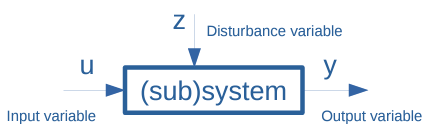
\includegraphics[width = 0.5 \textwidth]{Imagenes/1 - Block.png}
    \label{Fig: 1 - Block}
\end{figure}

\subsection{Closed Loop Control}
\subsubsection{Open Loop Control}
\begin{itemize}
    \item Simple and cheap
    \item Not useful in the presence of important model errors or distrubances
\end{itemize}

\begin{figure}[H]
    \centering
    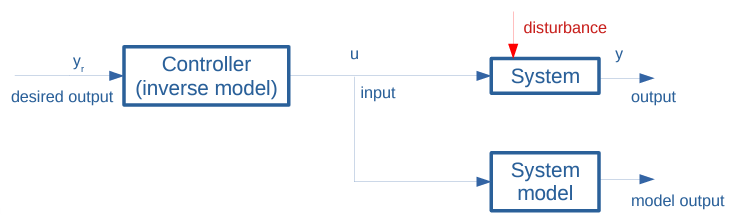
\includegraphics[width = 0.5 \textwidth]{Imagenes/1 - Open Loop Control.png}
    \label{Fig: 1 - Open Loop Control}
\end{figure}

\subsubsection{Closed Loop Control}
\begin{itemize}
    \item Robust in the presence of model errors
    \item Robust in the presence of distrubances
\end{itemize}

\begin{figure}[H]
    \centering
    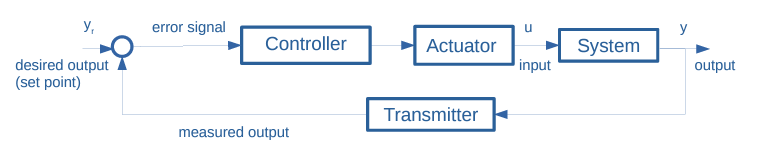
\includegraphics[width = 0.5 \textwidth]{Imagenes/1 - Closed Loop Control.png}
    \label{Fig: 1 - Closed Loop Control}
\end{figure}

Main features of Process Control:
\begin{itemize}
    \item System models are usually non-linear
    \item Processes are often stable and over-damped
    \item Delays play a vital role
    \item Improving the behavior in the presence of distrubances is more important than dealing with set point changes
\end{itemize}

\subsection{Process Control Methods}
Control systems may present one single loop (Basic Regulatory control or BRC Control) or several closed loops (Cascade-based Advanced Control). Other advanced control schemes that we will see are: Feed Forward Control and the Smith Predictor.

\section{P\&ID}
P\&ID Representation of Processes:
\begin{itemize}
    \item P\&ID: Piping and Instrimentation Diagram
    \item International notation, essential to specify and deploy the industrial control systems layout
\end{itemize}

\begin{figure}[H]
    \centering
    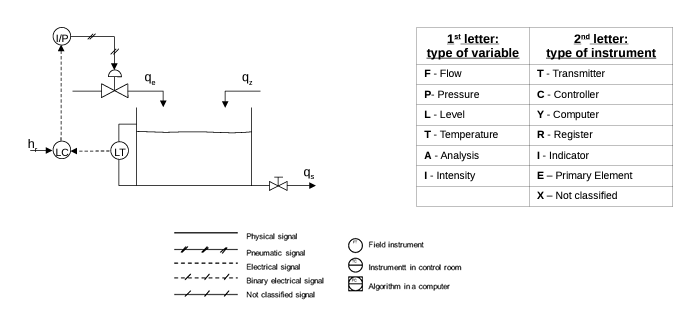
\includegraphics[width = 0.5 \textwidth]{Imagenes/1 - PID Representation.png}
    \label{Fig: 1 - PID Representation}
\end{figure}

Different types of valves have different P\&ID representations
\begin{figure}[H]
    \centering
    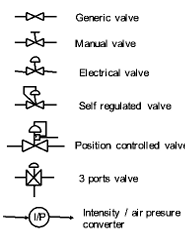
\includegraphics[width = 0.25 \textwidth]{Imagenes/1 - PID Valve Representation.png}
    \label{Fig: 1 - PID Valve Representation}
\end{figure}